\documentclass[12pt]{article}
\usepackage{amsmath}
\usepackage{verbatim}
\usepackage{subfigure}
\usepackage[pdftex]{graphicx}


 \topmargin -1.5cm        % read Lamport p.163
 \oddsidemargin -1.04cm   % read Lamport p.163
 \evensidemargin -1.04cm  % same as oddsidemargin but for left-hand pages
 \textwidth 18.59cm
 \textheight 21.94cm 
 
\begin{document}

\title{Benchmarking the Isorropia LevelSolver Class on a Multi-core Node}
\author{C. G. Baker, E. G. Boman, C. Chevalier, \\ M. A. Heroux, L. A. Riesen}
\date{Tuesday, July 21, 2009}
\maketitle

\section{Introduction}

This document archives the initial benchmarking of the Isorropia \texttt{LevelSolver} class, as well as some analysis of the performance on a multi-core CPU node. The purpose of the \texttt{LevelSolver} class is to exploit the level-set analysis capability of Isorropia and the parallel linear algebra capability of Kokkos in order to provide a parallel triangular matrix solve. This is accomplished by partitioning the rows of a lower triangular matrix into a number of ``level-sets.'' This partitioning comes via a level-set analysis of the matrix structure, which exploits sparsity in the matrix in order to expose parallelism typically unavailable in the forward-substition solution of a dense lower-triangular matrix.

For example, consider a non-singular lower triangular matrix $L$. Assume the existence of a permutation matrix $P$ such that $\hat{L} = P L P^T$ is another triangular matrix with the following block structure:
\[
\hat{L} = \begin{bmatrix} D_1    &               &             & \\
                     B_{21} & D_2     &             & \\
                B_{31} & B_{32} & D_3     & \\
                 B_{41} & B_{42} & B_{43} & D_4
       \end{bmatrix}, 
\]
where each matrix $D_i$ is a diagonal matrix. This matrix has been permuted by $P$ to expose the existence of four levelsets. The solution of a linear system $L x = y$ can be computed as follows. Denoting $\hat{x} = P x$ and $\hat{y} = P y$, we can rewrite $L x = y$ as $\hat{L} \hat{x} = \hat{y}$. Partitioning $\hat{x}$ and $\hat{y}$ conformally with $\hat{L}$ and multiplying yields the following, and $x$ can be found via $P^T \hat{x}$:
\begin{align*}
D_1 \hat{x}_1 &= \hat{y}_1 \\
D_2 \hat{x}_2 &=  \hat{y}_2 - B_{21} \hat{x}_1 \\
D_3 \hat{x}_3 &= \hat{y}_3 - B_{31} \hat{x}_1 - B_{32} \hat{x}_2 \\
D_4 \hat{x}_4 &= \hat{y}_4 - B_{41} \hat{x}_1 - B_{42} \hat{x}_2 - B_{43} \hat{x}_3 
\end{align*}

For a general sparse matrix $\hat{L}$ partitioned as such, the solution can be written as follows:
\begin{verbatim}
Parameters: level sizes lsize[i], numLevels
Input: vectors x, y
ptr = 1
for i=1:numLevels,
   if i > 1,
      y(ptr:ptr+lsize(i)) -= B(i,:) * x(1:ptr-1)
   endif
   x(ptr:ptr+lsize(i)) = D(i) \ y(ptr:ptr+lsize(i))
   ptr = ptr + lsize(i)
endfor
\end{verbatim}

This process can be thought of as a type of block forward-substition algorithm. However, unlike a typical block triangular solve, the level set analysis results in diagonal blocks $D_i$ which are themselves diagonal. This makes explicit the mutual independence of the rows of $\hat{x}$ inside a given level; i.e., the entries of $\hat{x}$ in level $i$ depend on the on the (already computed) entries of $\hat{x}$ from previous levels, so that each of these entries can be computed independent from (and more importantly, parallel to) the other entries. Contrast this to a block forward-substituion solve without the benefit of the level-set analysi: there, the blocks $D_i$ are not diagonal, and therefore they couple the entries in $\hat{x}_i$. 

The solution of the triangular system becomes a sequence of sparse matrix-vector products and diagonal scalings, each of which can potentially be parallelized. As long as there is sufficient work inside a level (i.e., sufficient non-zeros to amortize the overhead associated with the level set analysis and partitioning), parallelization of the individual levels can result in a speedup over a standard forward-substitution triangular solve.

\section{\texttt{LevelSolver} Class Organization}

The \texttt{LevelSolver} class currently exists in Isorropia. This class inherits from abstract base class \texttt{Epetra\_Operator}, implementing methods \texttt{Apply()} and \texttt{AppyInverse()} to solve or multiply a triangular system, respectively. The class provides two methods specific to the operation of the level-set solvers: \texttt{Analyze()} accepts an \texttt{Epetra\_CrsGraph} object specifying the non-zero structure for the triangular matrix to undergo level-set analysis; and \texttt{Setup()} accepts an \texttt{Epetra\_CrsMatrix} object containing the values of the lower-triangular matrix. 

The \texttt{LevelSolver} class stores two primary groups of information: the level-set information (level sizes and permutation matrix $P$), and data structures for the partition blocks $D_i$ and $B_i$ comprising $\hat{L}$ (the sub-diagonal blocks associated with a particular level are stored in a single sparse matrix). The entire diagonal block is represented as a one-dimensional array, while each sub-diagonal block $B_i$ is stored in a local (i.e., non-distributed) \texttt{Kokkos::SparseMatVec} object.\footnote{The contents of a sparse matrix block $B_i$ are temporarily stored in a \texttt{Kokkos::SparseMatrix} object, which is consumed by a \texttt{Kokkos::SparseMatVec} object. This is because the sparse matrix and the implementation of a sparse mat-vec are decoupled in Kokkos, and \texttt{LevelSolver} only needs the ability to affect the sparse mat-vec. The consequence is that the entries of the sparse matrix cannot be recovered from the \texttt{LevelSolver} objects; we can only experience $\hat{L}$ via multiplication or inversion.} 


\begin{figure}[htbp]
     \centering
      \subfigure{ %\label{lbl}
          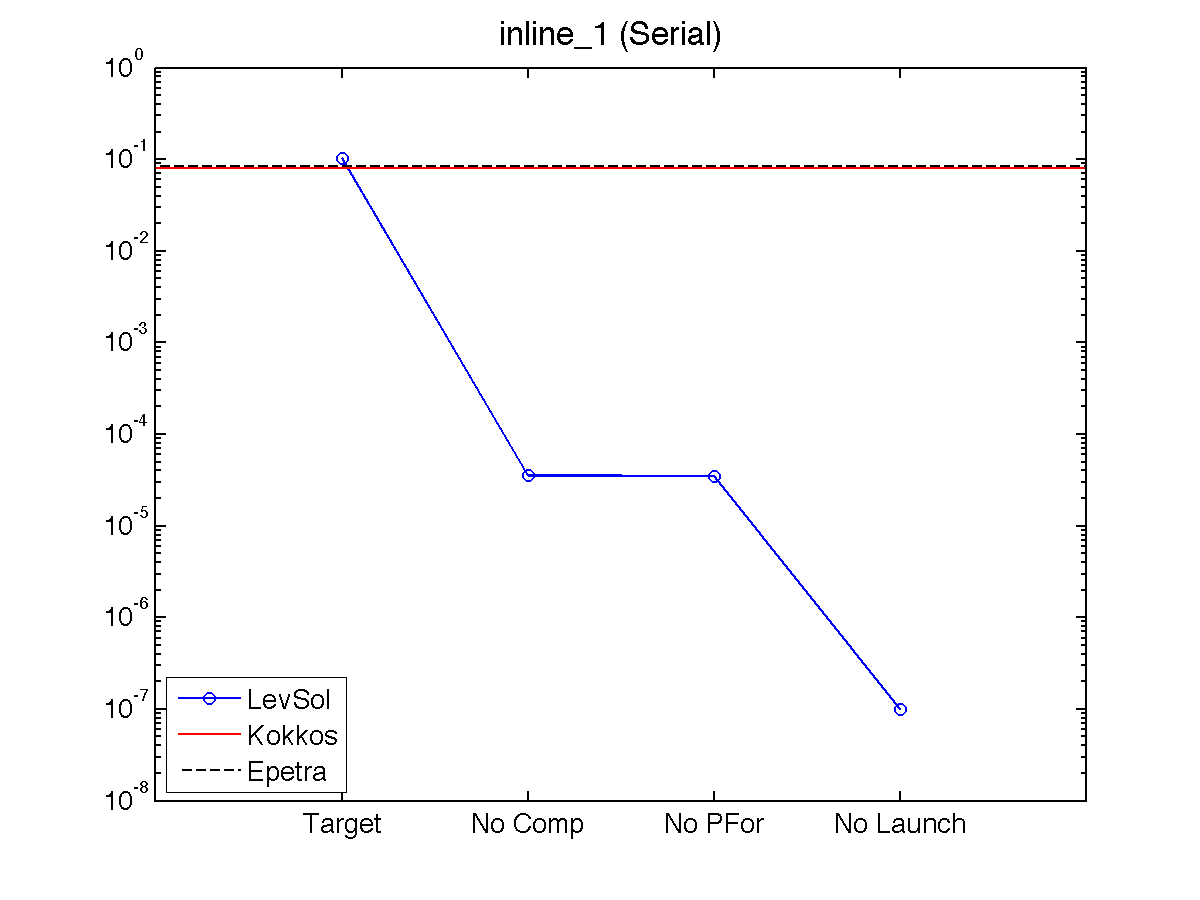
\includegraphics[width=9.05cm]{data/inline_1_serial.png}}
      \subfigure{ %\label{lbl}
          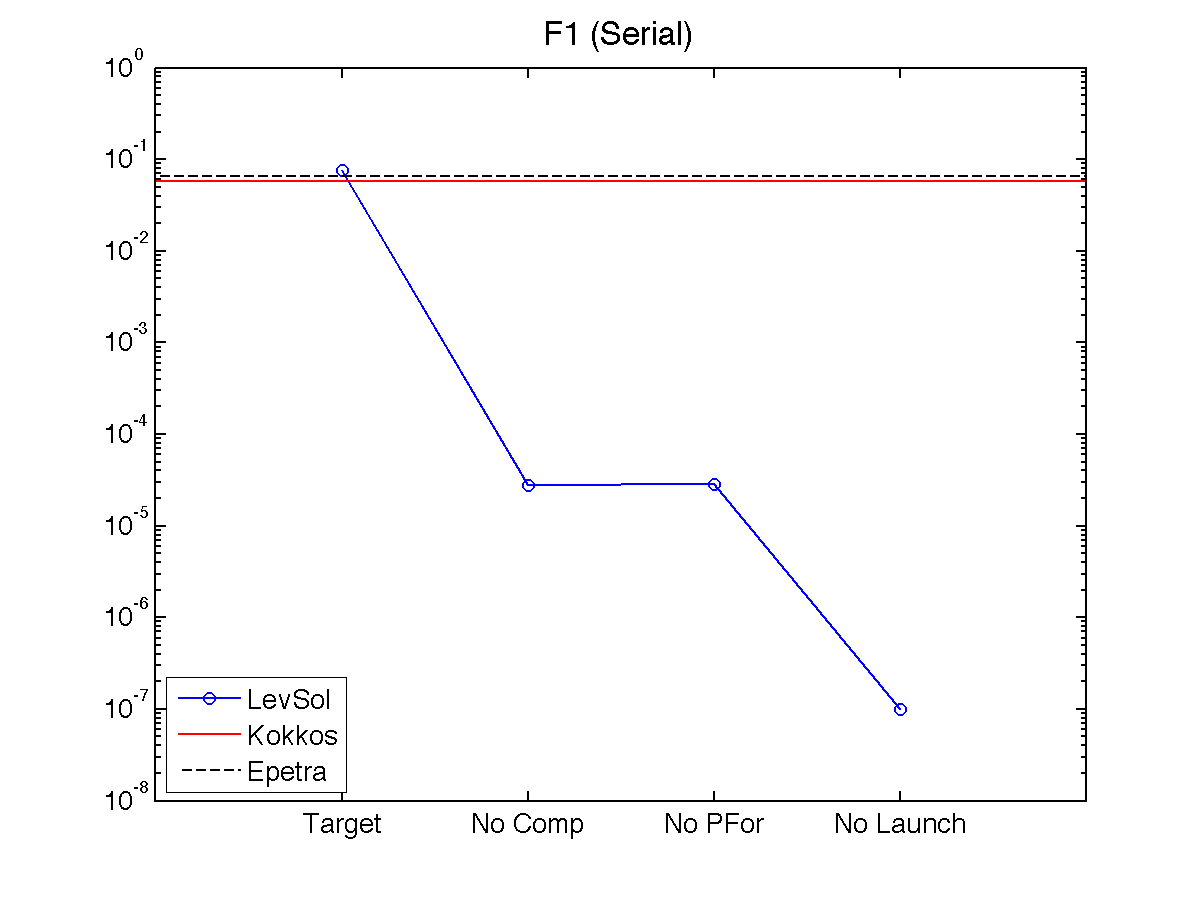
\includegraphics[width=9.05cm]{data/F1_serial.png}}
      \subfigure{ %\label{lbl}
          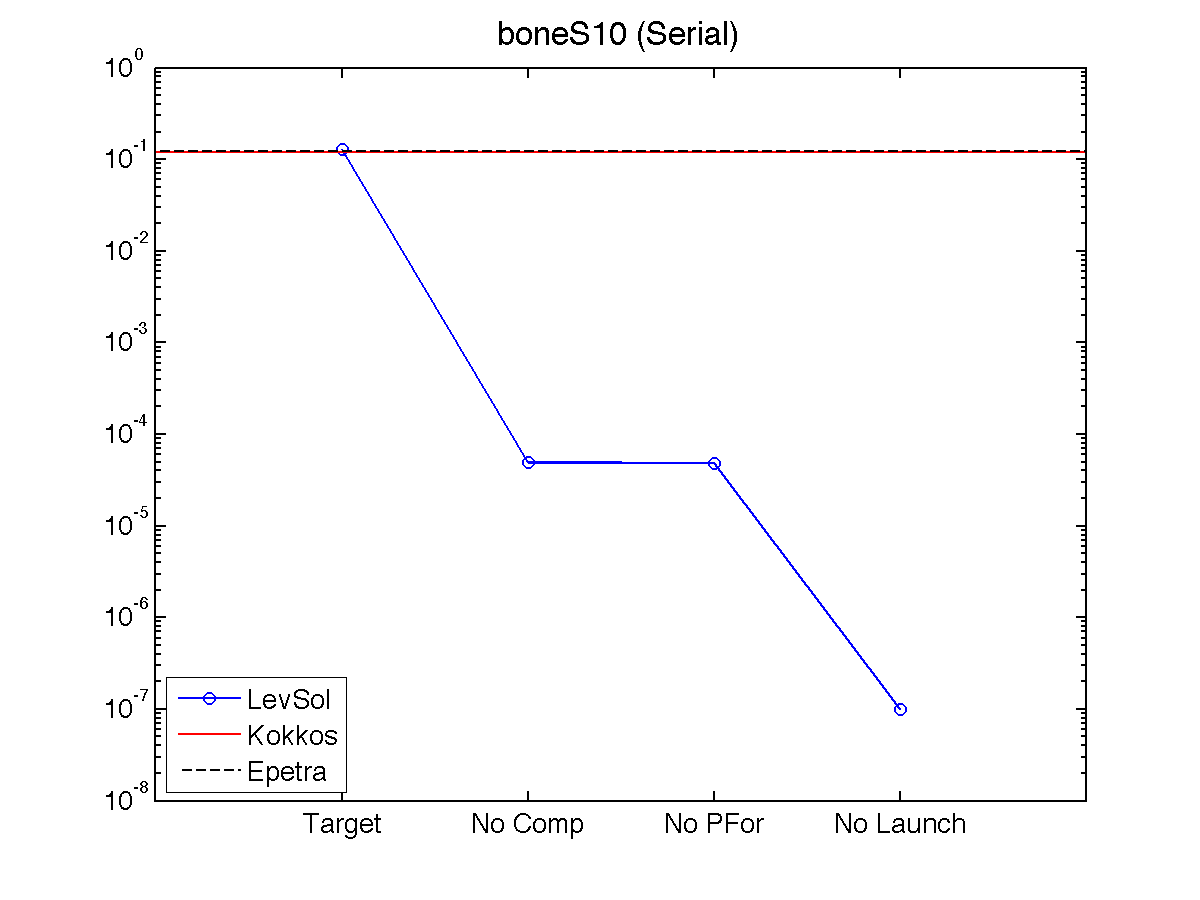
\includegraphics[width=9.05cm]{data/boneS10_serial.png}}
      \subfigure{ %\label{lbl}
          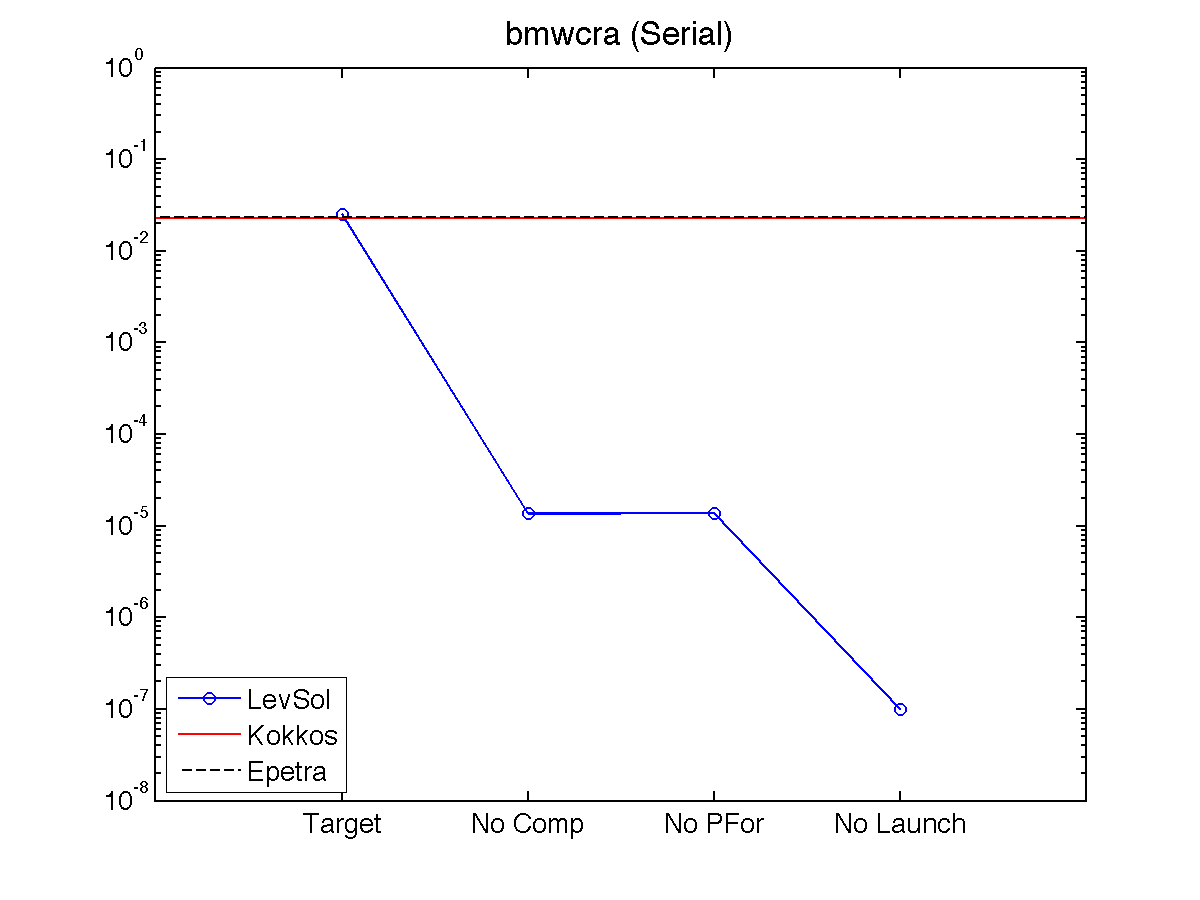
\includegraphics[width=9.05cm]{data/bmwcra_serial.png}}
      \subfigure{ %\label{lbl}
          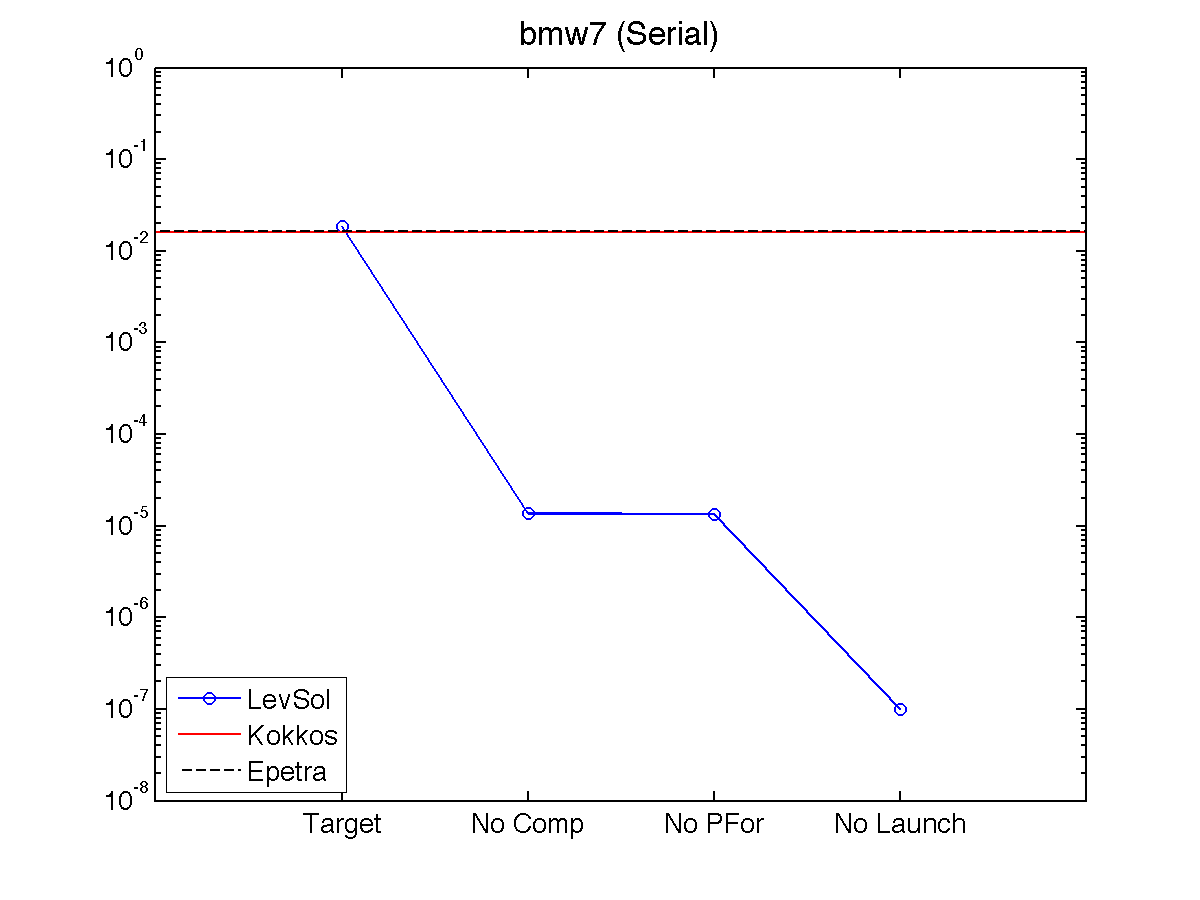
\includegraphics[width=9.05cm]{data/bmw7_serial.png}}
      \subfigure{ %\label{lbl}
          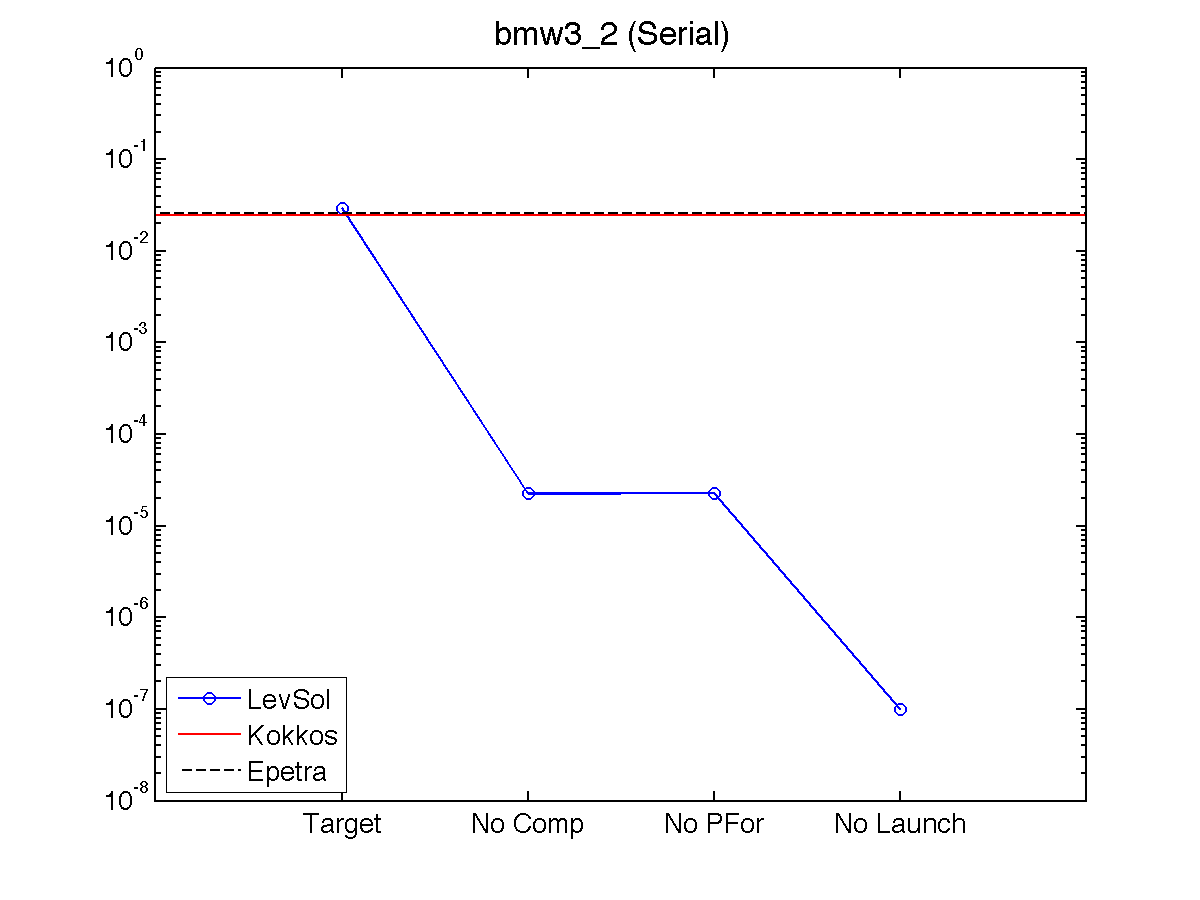
\includegraphics[width=9.05cm]{data/bmw3_2_serial.png}}
\caption{Results for serial node.}
\label{lbl:serialfigs}
\end{figure}


\begin{figure}[htbp]
     \centering
      \subfigure{ %\label{lbl}
          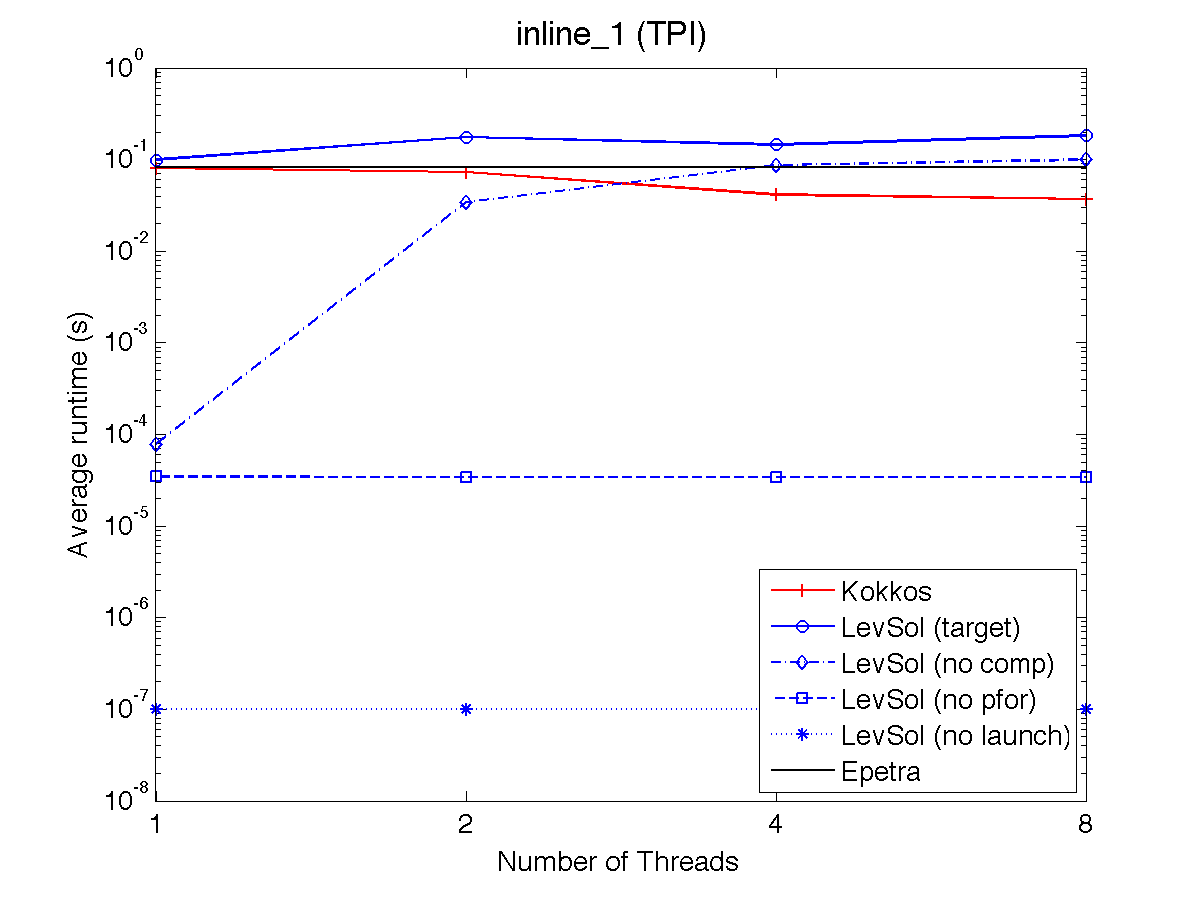
\includegraphics[width=9.05cm]{data/inline_1_tpi.png}}
      \subfigure{ %\label{lbl}
          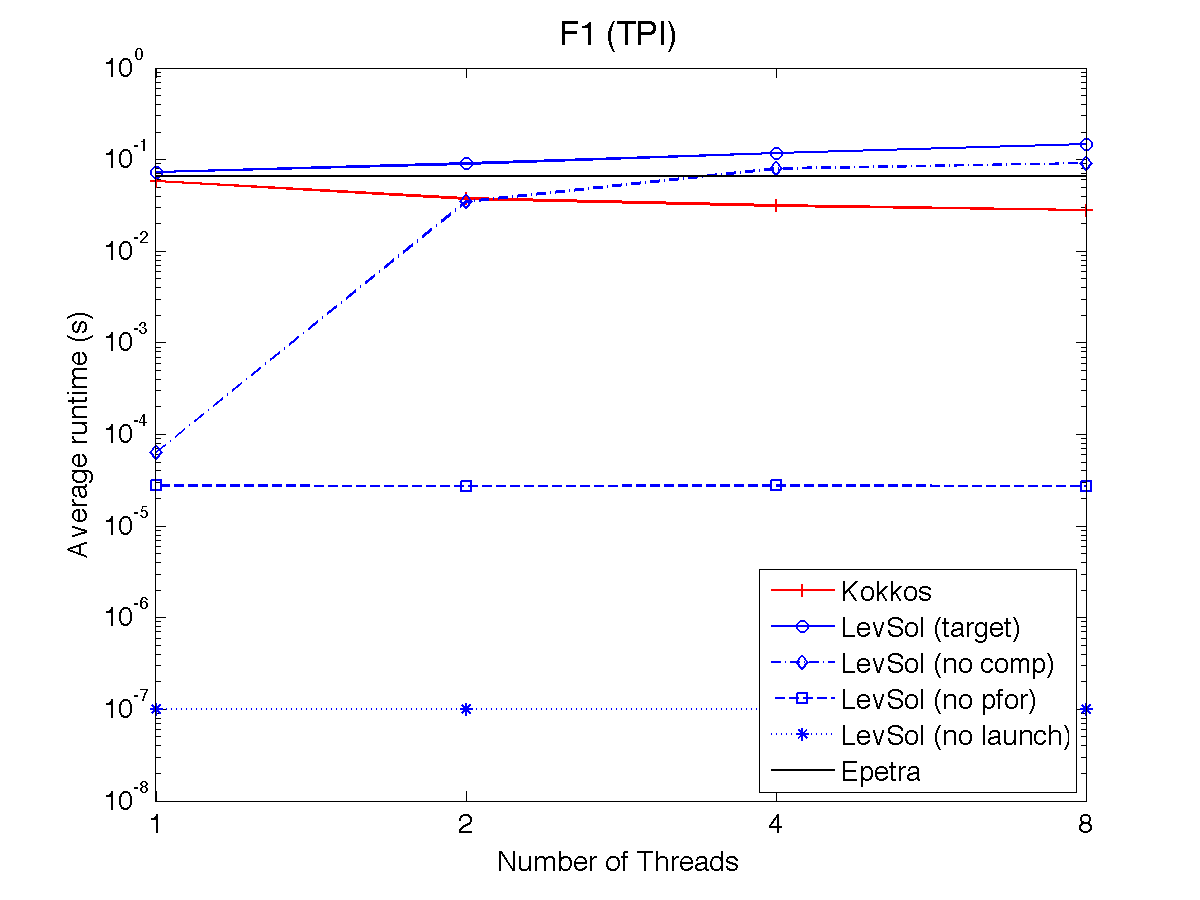
\includegraphics[width=9.05cm]{data/F1_tpi.png}}
      \subfigure{ %\label{lbl}
          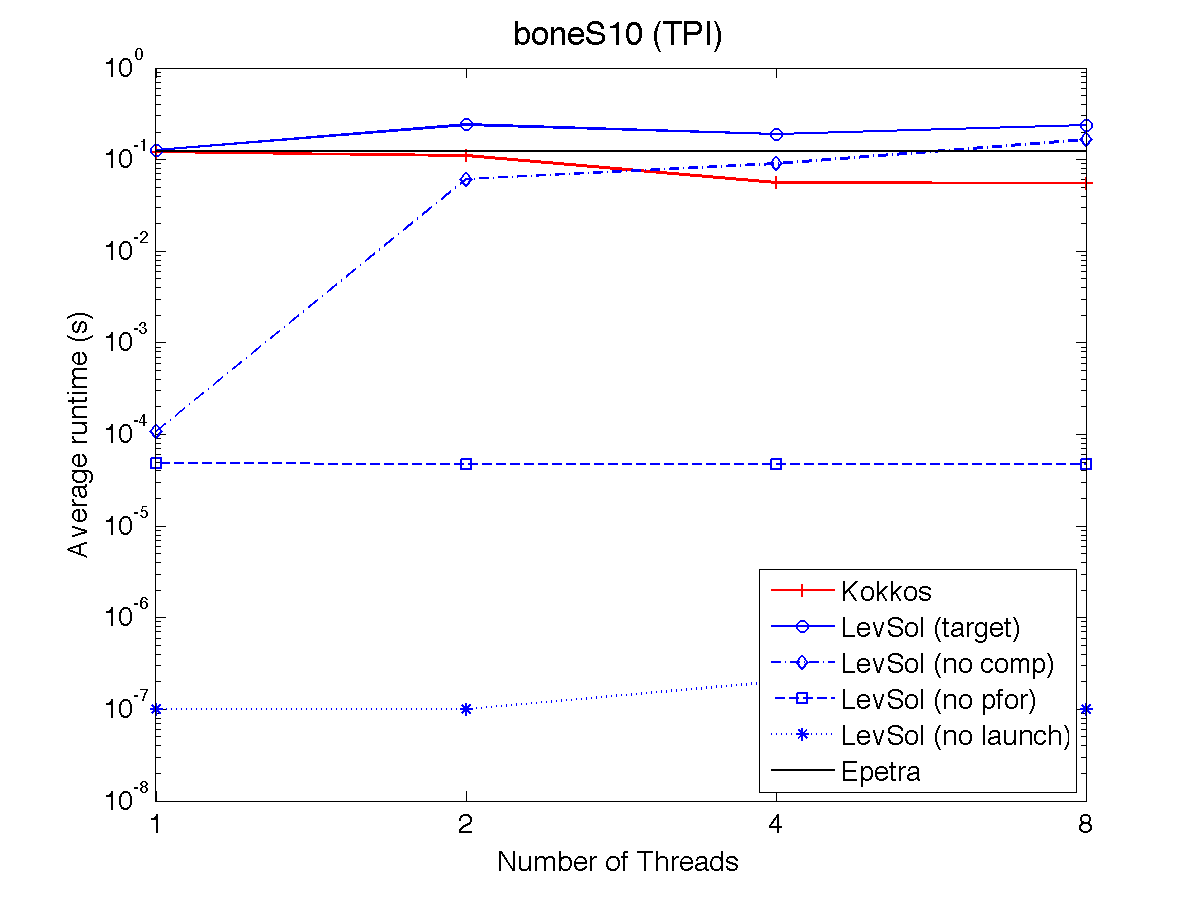
\includegraphics[width=9.05cm]{data/boneS10_tpi.png}}
      \subfigure{ %\label{lbl}
          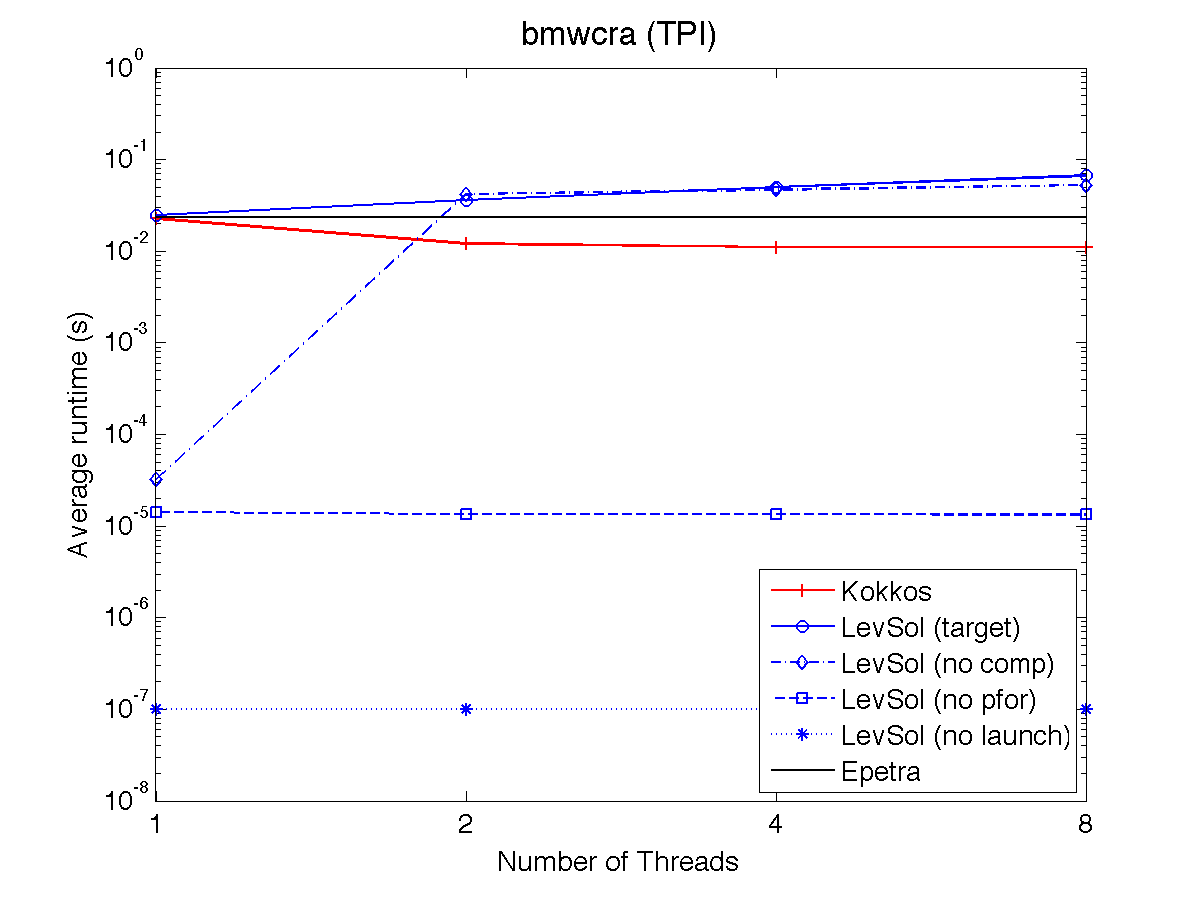
\includegraphics[width=9.05cm]{data/bmwcra_tpi.png}}
      \subfigure{ %\label{lbl}
          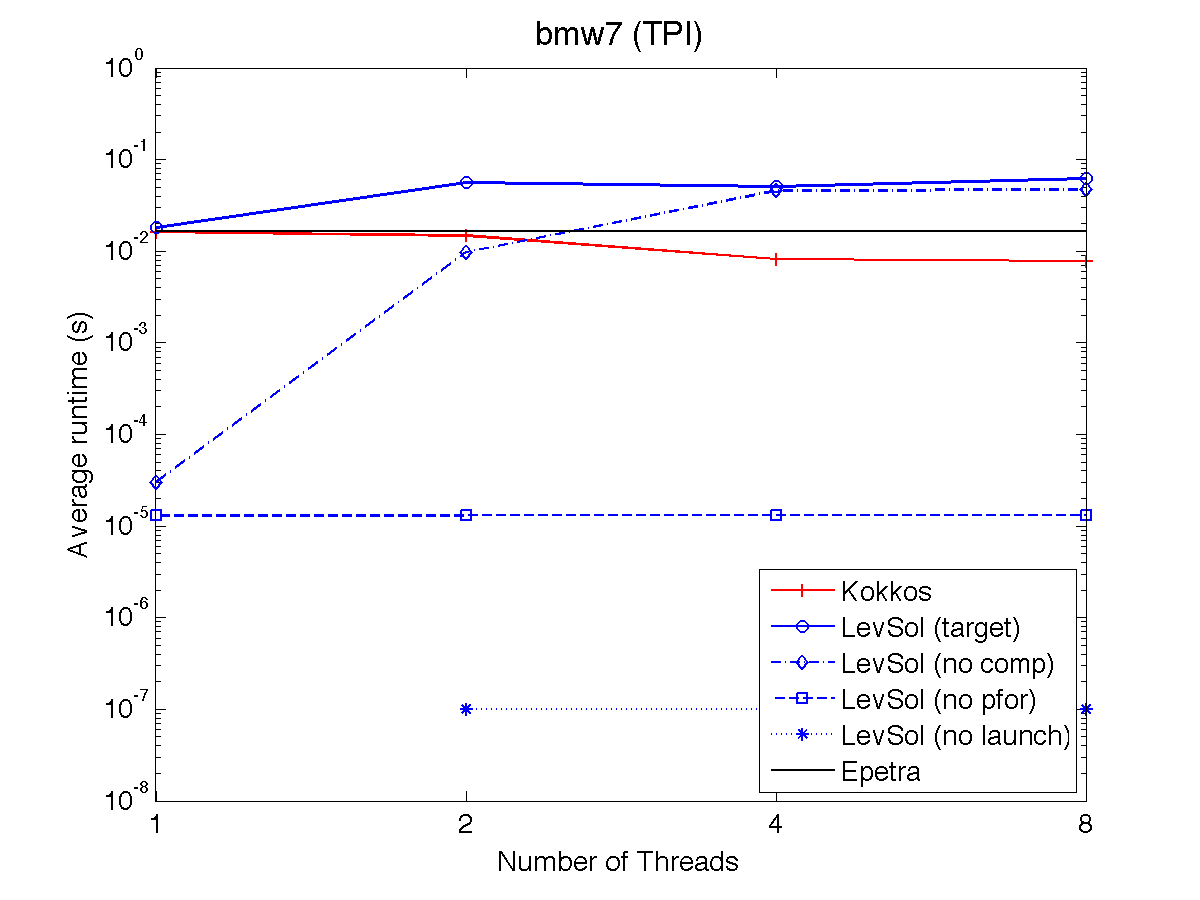
\includegraphics[width=9.05cm]{data/bmw7_tpi.png}}
      \subfigure{ %\label{lbl}
          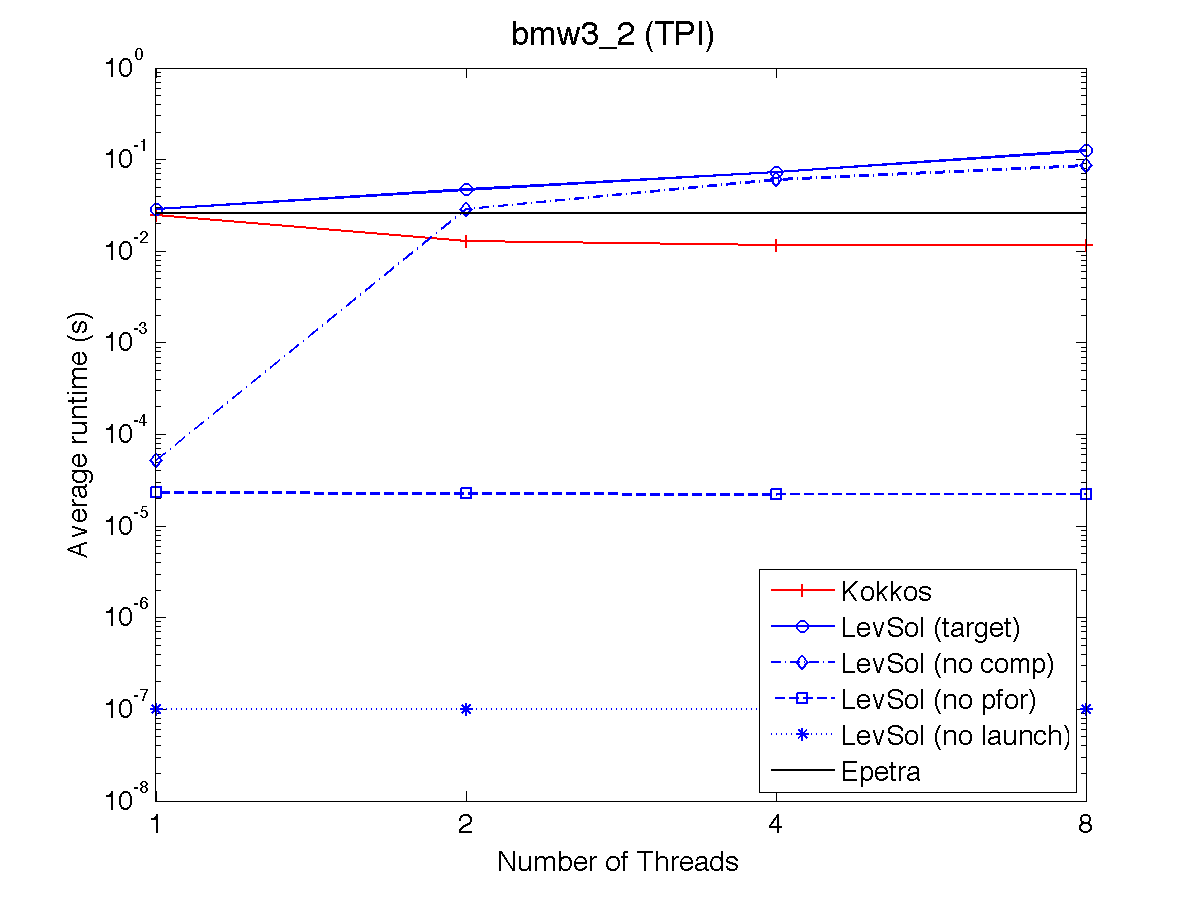
\includegraphics[width=9.05cm]{data/bmw3_2_tpi.png}}
\caption{Results for TPI node.}
\label{lbl:tpifigs}
\end{figure}


\begin{figure}[htbp]
     \centering
      \subfigure{ %\label{lbl}
          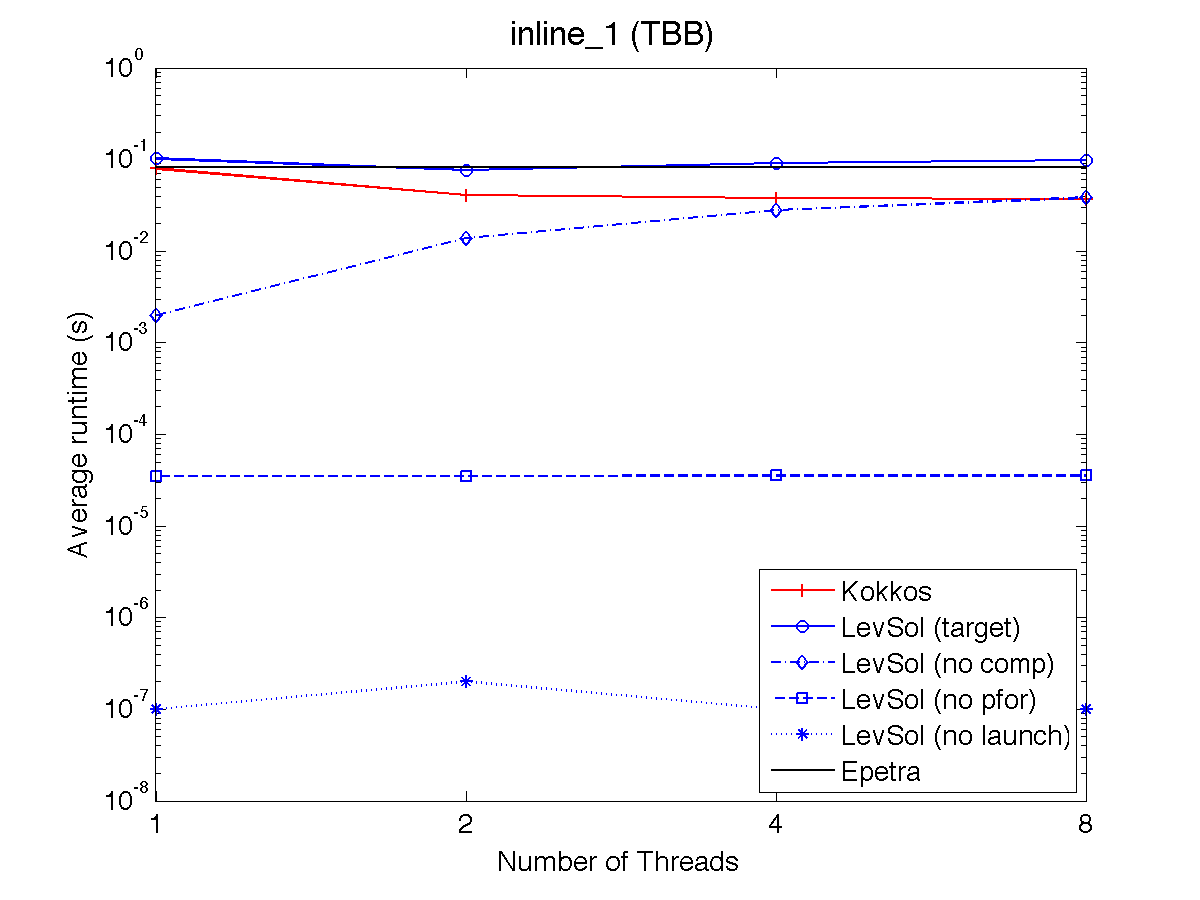
\includegraphics[width=9.05cm]{data/inline_1_tbb.png}}
      \subfigure{ %\label{lbl}
          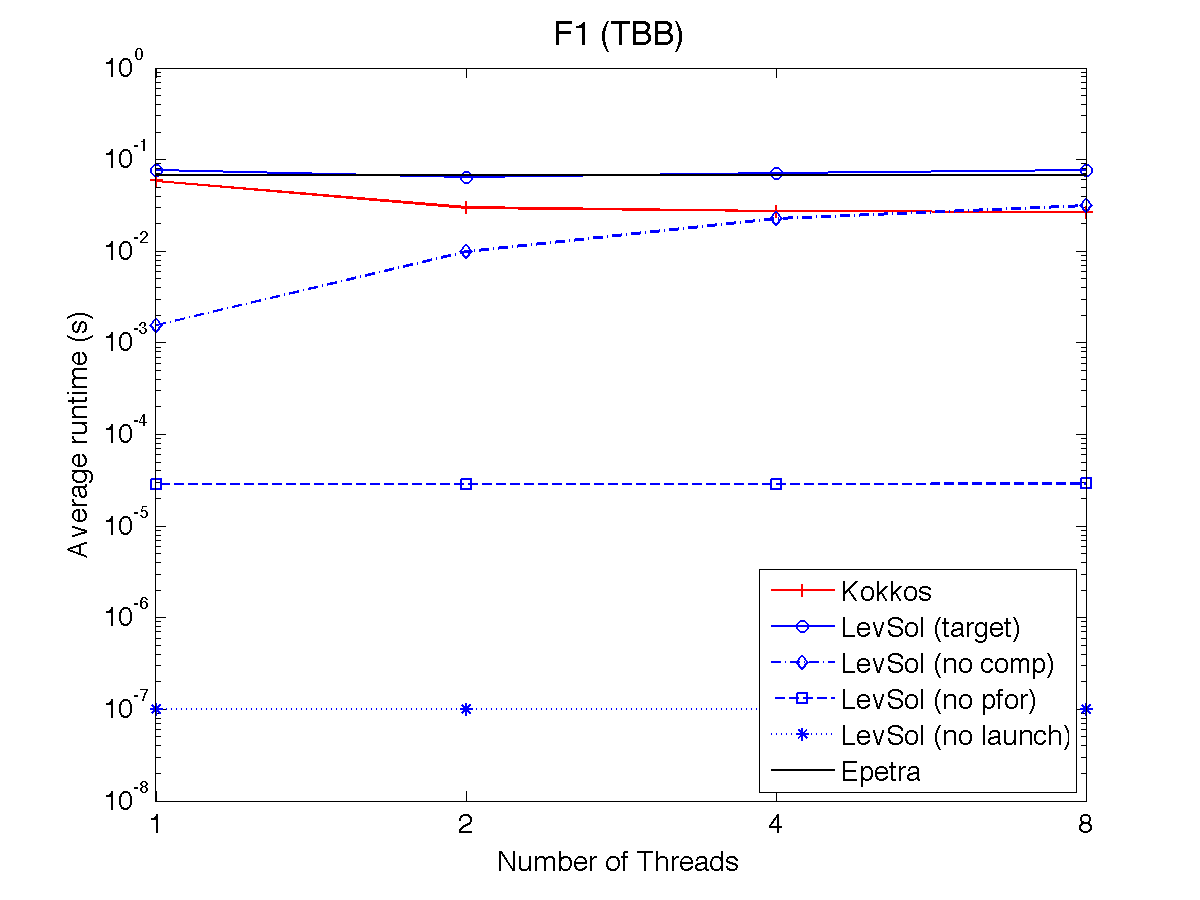
\includegraphics[width=9.05cm]{data/F1_tbb.png}}
      \subfigure{ %\label{lbl}
          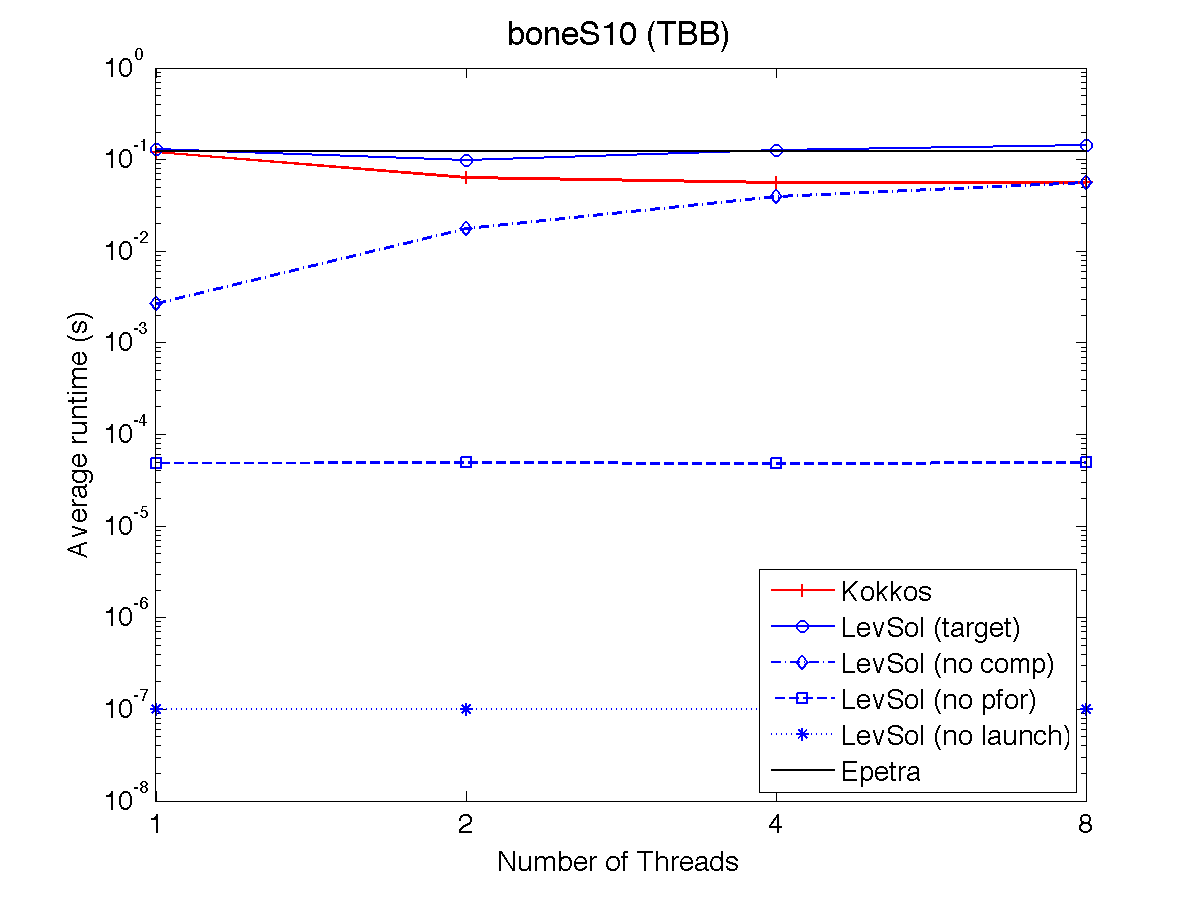
\includegraphics[width=9.05cm]{data/boneS10_tbb.png}}
      \subfigure{ %\label{lbl}
          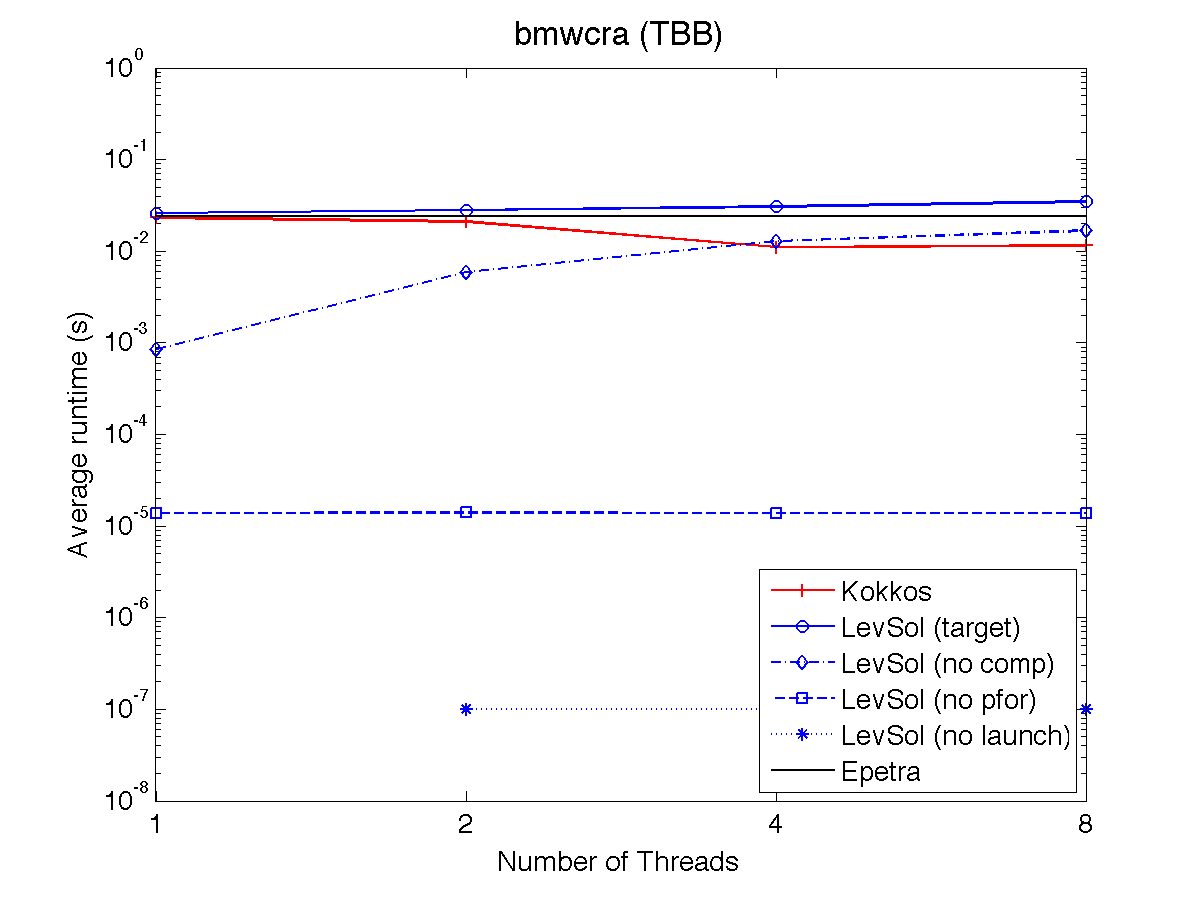
\includegraphics[width=9.05cm]{data/bmwcra_tbb.png}}
      \subfigure{ %\label{lbl}
          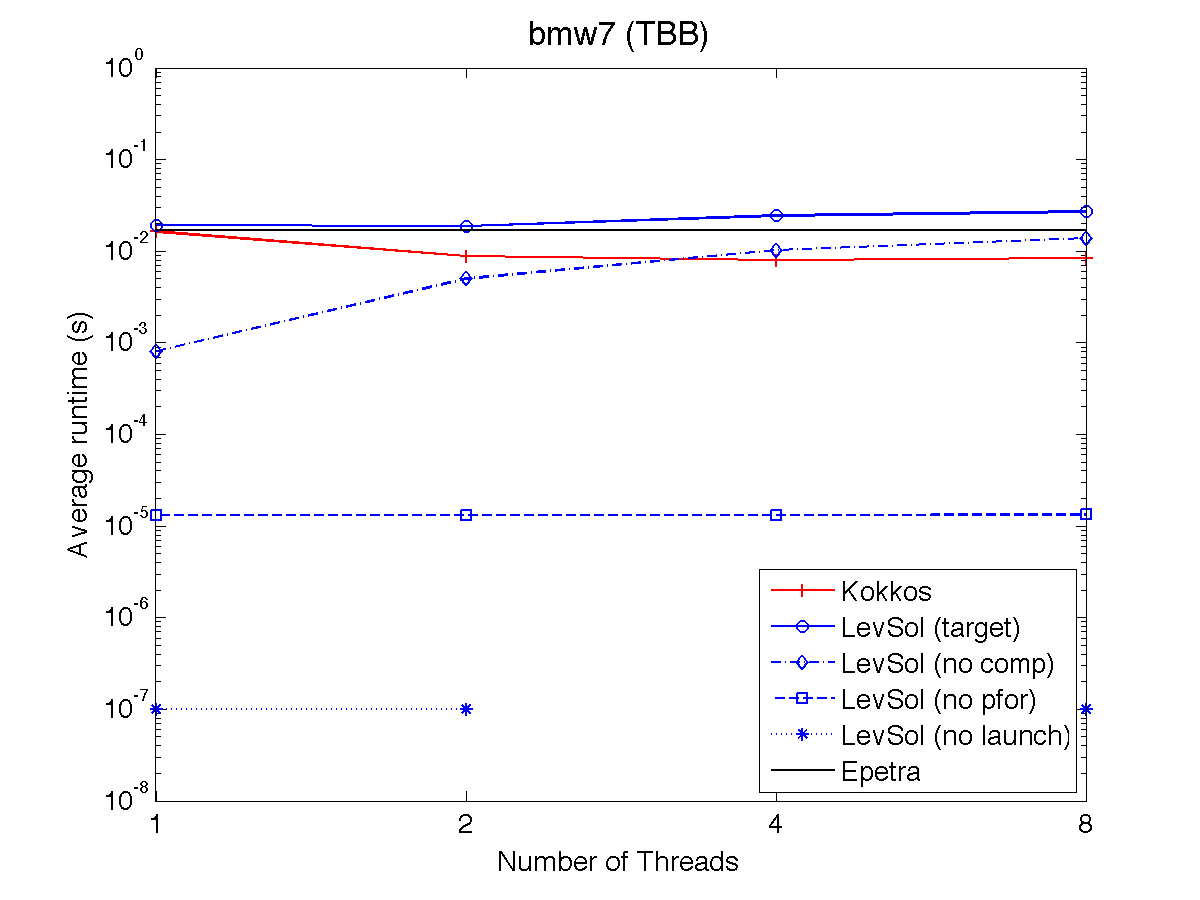
\includegraphics[width=9.05cm]{data/bmw7_tbb.png}}
      \subfigure{ %\label{lbl}
          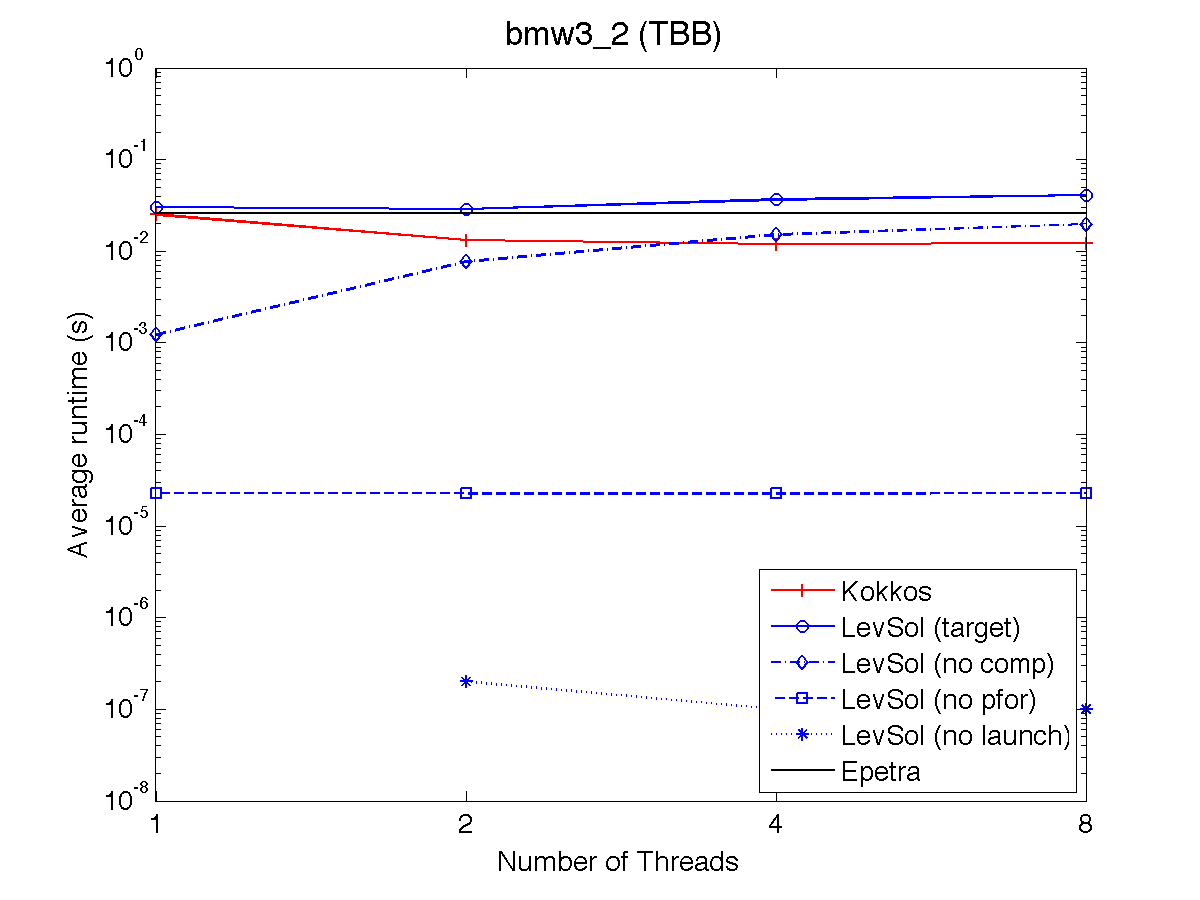
\includegraphics[width=9.05cm]{data/bmw3_2_tbb.png}}
\caption{Results for TBB node.}
\label{lbl:tbbfigs}
\end{figure}



\end{document}
